\documentclass{article}
\usepackage[utf8]{inputenc}
\usepackage{ctex}
\usepackage{amsmath}
\usepackage{float}
\usepackage{natbib}
\usepackage{graphicx}

\title{随机过程大作业}
\author{张栩萌 \ 519070910031}
\date{May 2022}



\begin{document}

\maketitle

\section{实验目的}
1. 通过计算机模拟布朗运动,观察布朗运动的特性

2. 通过计算机模拟随机微分方程解的轨道,探究不同参数对轨道的影响,计算机模拟$X_1$的期望和方差

3. 熟练Python编程建模操作




\section{问题一:布朗运动}
布朗运动的定义为:若一个随机过程$\{X(t), t \ge 0\}$满足\\
$X(t)$ 是独立增量过程;\\
$\forall s, t>0, X(s+t)-X(s) \sim N\left(0, c^{2} t\right)$, 即 $X(t+s)-X(s)$ 是数学期望 为 0 , 方差为 $c^{2} t$ 的正态分布;\\
$X(t)$ 关于 $t$ 是连续函数,\\
则称 $\{X(t), t \ge 0\}$ 是布朗运动或维纳过程. 当 $c=1$ 时, 称 $\{X(t), t \ge 0\}$ 是标准布朗运动。

图\ref{fig:brown1}为在$[0, 1]$区间生成100个等距点,以0.1为时间间隔生成的标准布朗运动,图\ref{fig:brown1_10}为同样的区间节点下生成的$c=10$时的布朗运动。

\begin{figure}[H]
    \centering
    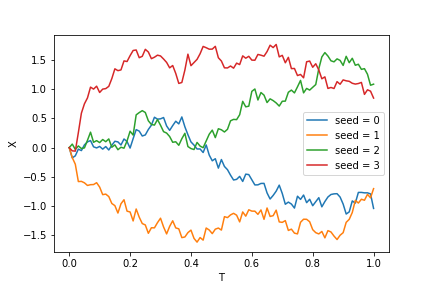
\includegraphics[scale=.6]{E:/Github/CourseWork/StochasticLearning/figs/多条布朗运动轨道.png}
    \caption{多条标准布朗运动轨道}
    \label{fig:brown1}
    \end{figure}

\begin{figure}[H]
    \centering
    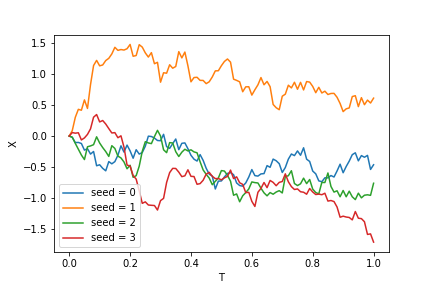
\includegraphics[scale=.6]{E:/Github/CourseWork/StochasticLearning/figs/多条布朗运动轨道c=10.png}
    \caption{当$c=10$时多条布朗运动轨道}
    \label{fig:brown1_10}
    \end{figure}

因为参数$c$影响布朗运动的增量正态分布的方差,所以我们看到当$c=10$时布朗运动振荡的幅度明显大于标准布朗运动。




\section{问题二:股票价值随机微分方程}
设 $B=\left\{B_{t} ; t \geq 0\right\}$ 为标准布朗运动, $X=\left\{X_{t} ; t \geq 0\right\}$ 为如下随机微分方程的解:
$$
\left\{\begin{array}{l}
d X_{t}=\alpha\left(v-X_{t}\right) d t+\sigma d B_{t} \\
X_{0}=x_{0}
\end{array}\right.
$$
其中 $\alpha, v, \sigma, x_{0}$ 为常数。



\section{问题三:股票价值与价格随机微分方程}





\section{总结}







\bibliographystyle{plain}
\bibliography{references}
\end{document}